\chapter{Case Studies}

An application's user is generally not happy about seeing advertisements in the application. They degrade the overall experience and distract from the contents of the application itself. However, for some developers, advertisements are the only way to monetize their application.

In this chapter we try to determine how the proposed advertising methods compares to the more traditional ones in terms of user experience.

\section{Validation}

\textbf{Setup and Methodology:} To validate the hypothesis, the proposed solution is compared to traditional advertisement frameworks in terms of intrusiveness and effectiveness. A use case based on a Wikipedia app \footnote{https://github.com/wikimedia/WikipediaMobile} is developed, which implements the advertising library. This application is selected because the mechanism targets applications that present content to the user such as news, feeds, text, etc.

Initially, we integrate  traditional advertisement mechanisms into the selected application as shown in Figure \ref{fig:ads1}.

Next, we use the same Wikipedia application, but this time with our proposed solution implemented as seen in Figures \ref{fig:ads2} and \ref{fig:ads3}.


\begin{figure}
\begin{center}

\includegraphics[scale=0.25]{Images/classicalad_banner.png}

\includegraphics[scale=0.25]{Images/classicalad_fullscreen.png}
\caption{Examples of the application a banner or full screen advertisement}
\label{fig:ads1}
\end{center}
\end{figure}

Figure 5.2 shows what the application might look like right after a \textit{Gestrure Ad} appears and how it might look like after the user moves it to finish their reading.

\begin{figure}
\begin{center}

\includegraphics[scale=0.25]{Images/gesturead_small1.png}

\includegraphics[scale=0.25]{Images/gesturead_small2.png}
\caption{Examples of the application with a \textit{Gestrure Ad} in minimised form displayed}
\label{fig:ads2}
\end{center}
\end{figure}

Figure 5.3 shows what the application might look like after the user zooms in on the advertisement and how it might look like after the user has started dragging it left to indicate disinterest in it.

\begin{figure}
\begin{center}

\includegraphics[scale=0.25]{Images/gesturead_big1.png}
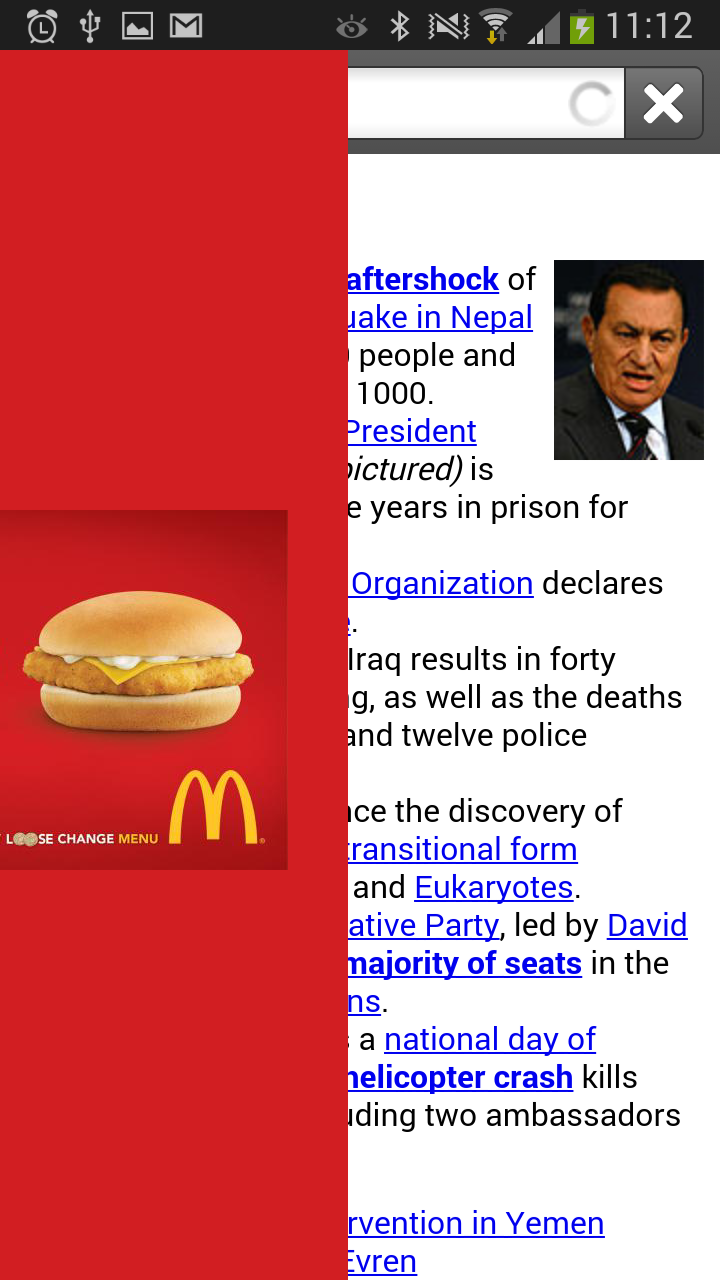
\includegraphics[scale=0.25]{Images/gesturead_big2.png}
\caption{Examples of the application with a \textit{Gestrure Ad} in maximised form displayed}
\label{fig:ads3}
\end{center}
\end{figure}

To measure how users view the proposed method, a questionnaire was composed. [Appendix A] It consists of 14 questions. 10 of the questions are about day-to-day application usage and opinion on traditional mobile advertisements. The final four questions are pertaining to the dynamic nature of the advertisement and how it compares to advertisements the participants are used to seeing in applications.

There were 25 participants between the ages of 20 and 35, all day-to-day smartphone users. 64\% of the participants were male.

They were asked to answer the first ten questions. Then they were asked to read an article of their choice from the Wikipedia application, half way though which an advertisement appeared, and asked to answer the final four questions.

\section{Results}

\subsection{Participants' Opinion on Traditional Mobile Advertising}

The participants claimed to be using their mobile devices anywhere between less than 30 minutes and more than 3 hours, however more than half of the participants use their mobile device 30 minutes to 1 hour each day as seen on Figure \ref{q1}.

\begin{figure}
\begin{center}
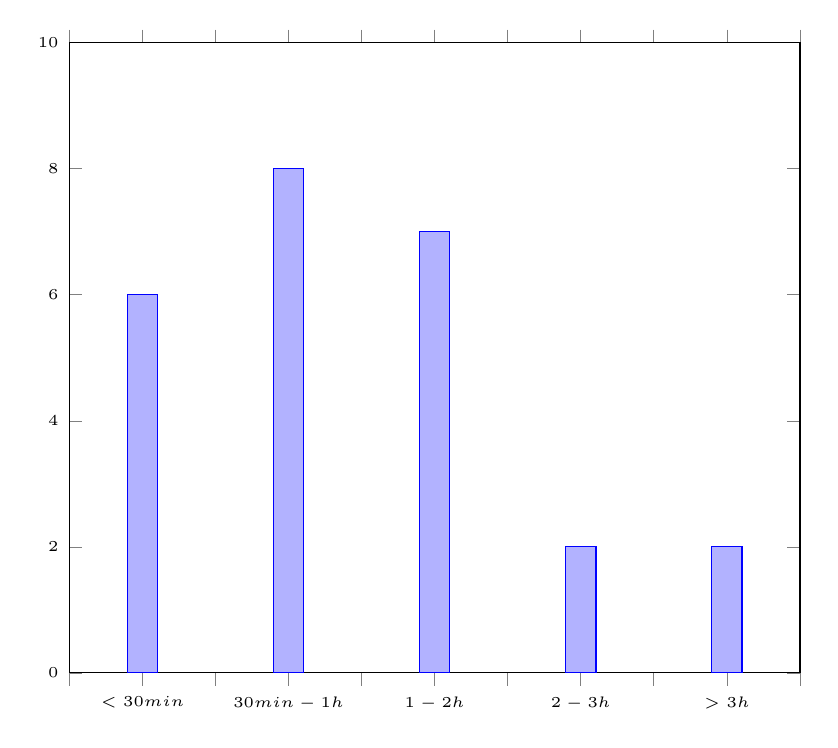
\begin{tikzpicture}[scale=1.1]

\begin{axis}[
style={font=\tiny},
ybar,
scale only axis,
xmin=0, xmax=20,
xticklabels={, ,$<30min$, ,$30min-1h$, ,$1-2h$, ,$2-3h$, ,$>3h$},
ymin=0, ymax=10,
]

\addplot coordinates{ (2,6) (6,8) (10,7) (14,2) (18,2)};

\end{axis}
\end{tikzpicture}
\caption{Participants' mobile device usage}
\label{q1}
\end{center}
\end{figure}

The average rating the participants gave to classical mobile advertisements bothering them is 3.72 on a scale from 1 to 5, 1 meaning not at all and 5 meaning very much. None of the participants claimed that mobile advertisements did not bother them at all as seen on Figure \ref{q2}. Many reasons were pointed out why advertisements are bothersome. The main ones being that the advertisements are distracting from using the application (flashing, sounds), take up a lot of screen space and are sometimes difficult or even impossible to get rid of.

\begin{figure}
\begin{center}
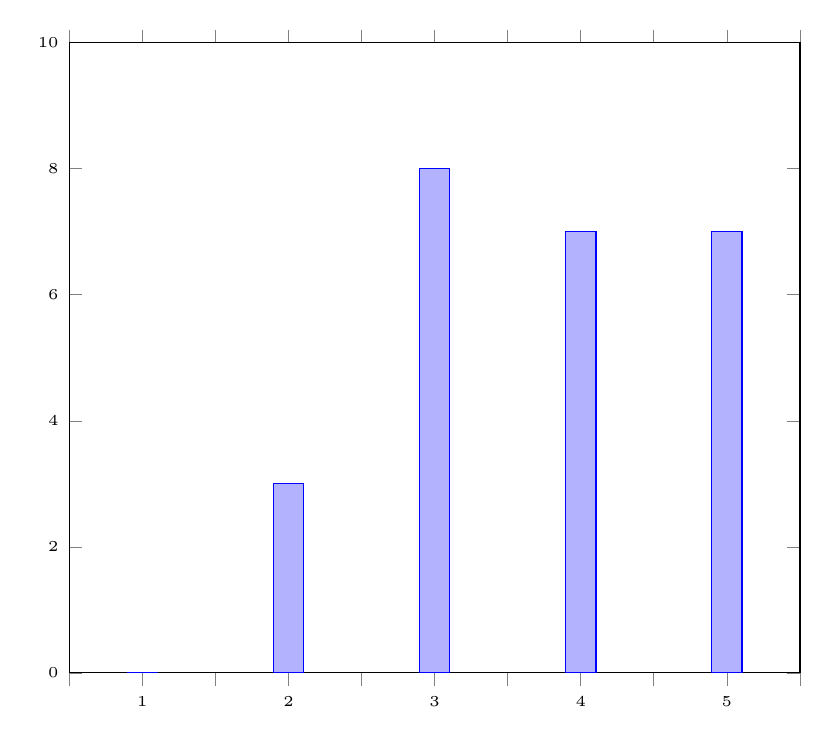
\begin{tikzpicture}[scale=1.1]

\begin{axis}[
style={font=\tiny},
ybar,
scale only axis,
xmin=0, xmax=20,
xticklabels={, ,$1$, ,$2$, ,$3$, ,$4$, ,$5$},
ymin=0, ymax=10,
]

\addplot coordinates{ (2,0) (6,3) (10,8) (14,7) (18,7)};

\end{axis}
\end{tikzpicture}
\caption{How much participants are bothered by advertisements in mobile applications}
\label{q2}
\end{center}
\end{figure}

Furthermore, 84\% of the participants claim to have uninstalled a mobile application just because of the intrusiveness of it's advertisements as seen on Figure \ref{q3}, while only 28\% claim to have looked up a product or service because of an advertisement in an application as seen on Figure \ref{q4} and only 8\% to have actually paid for a product or service they saw in an advertisement as seen on Figure \ref{q5}.

\begin{figure}
\begin{center}
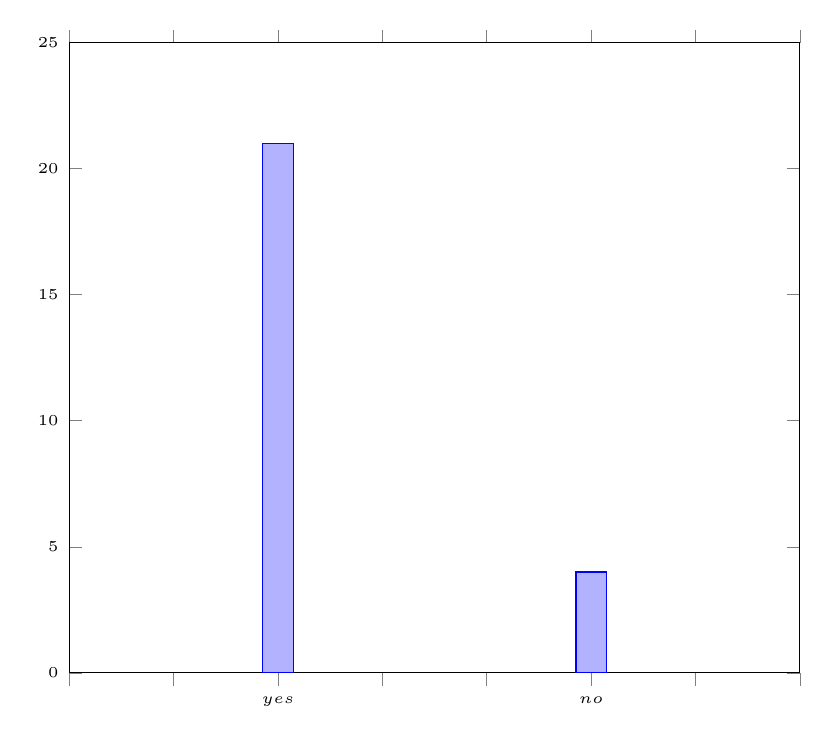
\begin{tikzpicture}[scale=1.1]

\begin{axis}[
style={font=\tiny},
ybar,
scale only axis,
xmin=0, xmax=3.5,
xticklabels={, , ,$yes$, , ,$no$},
ymin=0, ymax=25,
]

\addplot coordinates{ (1,21) (2.5,4) };

\end{axis}
\end{tikzpicture}
\caption{How many participants have uninstalled an application because of intrusive advertisements}
\label{q3}
\end{center}
\end{figure}

\begin{figure}
\begin{center}
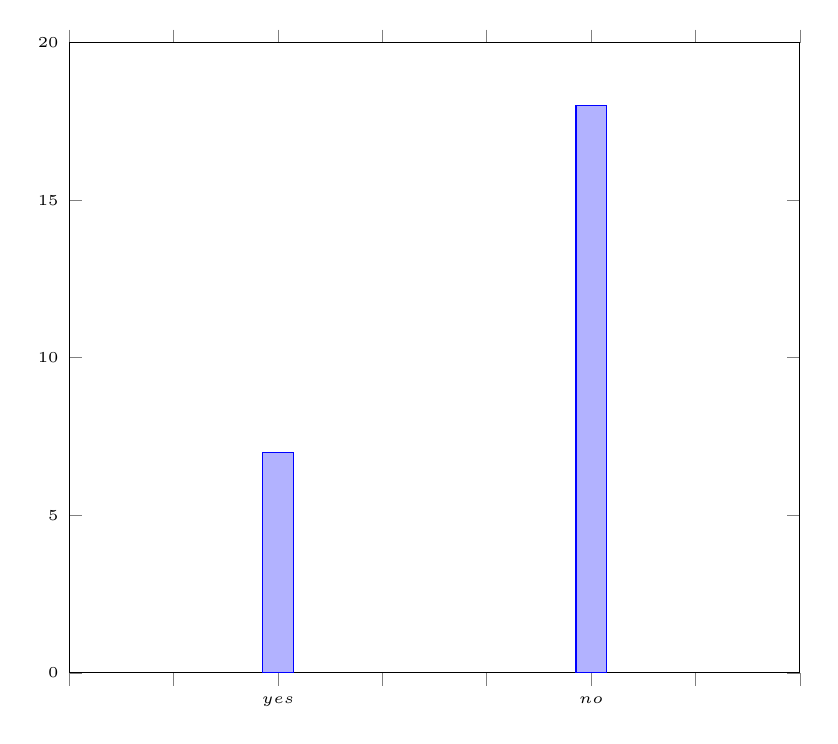
\begin{tikzpicture}[scale=1.1]

\begin{axis}[
style={font=\tiny},
ybar,
scale only axis,
xmin=0, xmax=3.5,
xticklabels={, , ,$yes$, , ,$no$},
ymin=0, ymax=20,
]

\addplot coordinates{ (1,7) (2.5,18) };

\end{axis}
\end{tikzpicture}
\caption{How many participants have looked up a product or a service because of a mobile advertisement}
\label{q4}
\end{center}
\end{figure}

\begin{figure}
\begin{center}
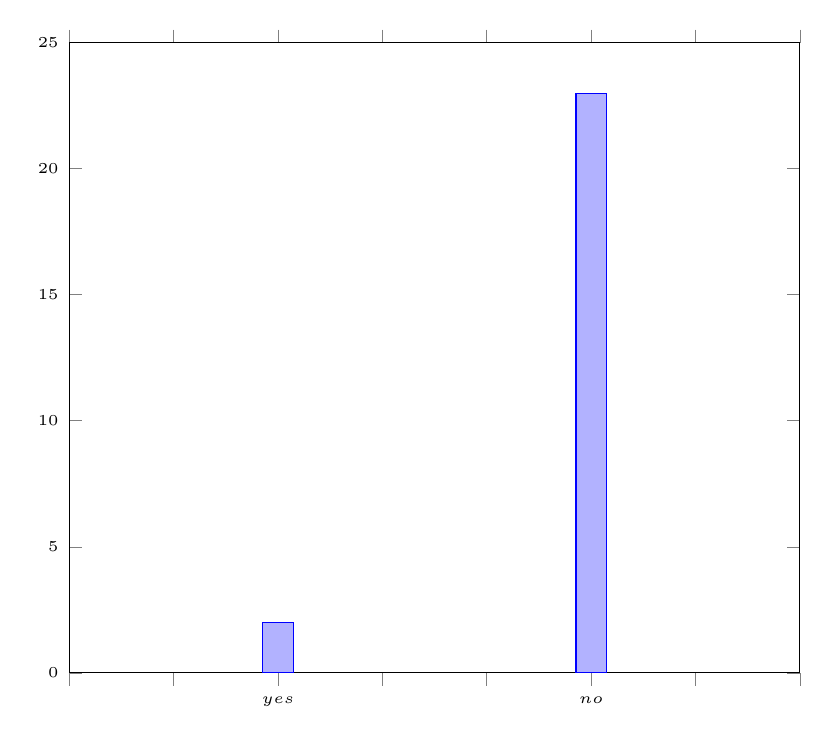
\begin{tikzpicture}[scale=1.1]

\begin{axis}[
style={font=\tiny},
ybar,
scale only axis,
xmin=0, xmax=3.5,
xticklabels={, , ,$yes$, , ,$no$},
ymin=0, ymax=25,
]

\addplot coordinates{ (1,2) (2.5,23) };

\end{axis}
\end{tikzpicture}
\caption{How many participants have paid for a product or a service because of a mobile advertisement}
\label{q5}
\end{center}
\end{figure}

This shows how ineffective traditional advertising methods are and that people are quite easily willing to stop using an application that has intrusive adverts. Traditional advertising methods are often quantity-over-quality and developers can easily damage their reputation without significant gain.

\subsection{Participants' Willingness to Adapt to New Methods of Advertising}

The participants were asked questions about their willingness to use functionality that this library provides without having used it before, to see whether they would be willing to adapt to dynamic advertisements in the applications they use.

All the participants thought they would get rid of an advertisement as soon as it appeared at least half the time as seen on Figure \ref{q6}, but 44\% of participants thought they would move an advertisement for later viewing at least some of the times and 24\% that they would want to view an advertisement later about half the times as seen on Figure \ref{q7}.

\begin{figure}
\begin{center}
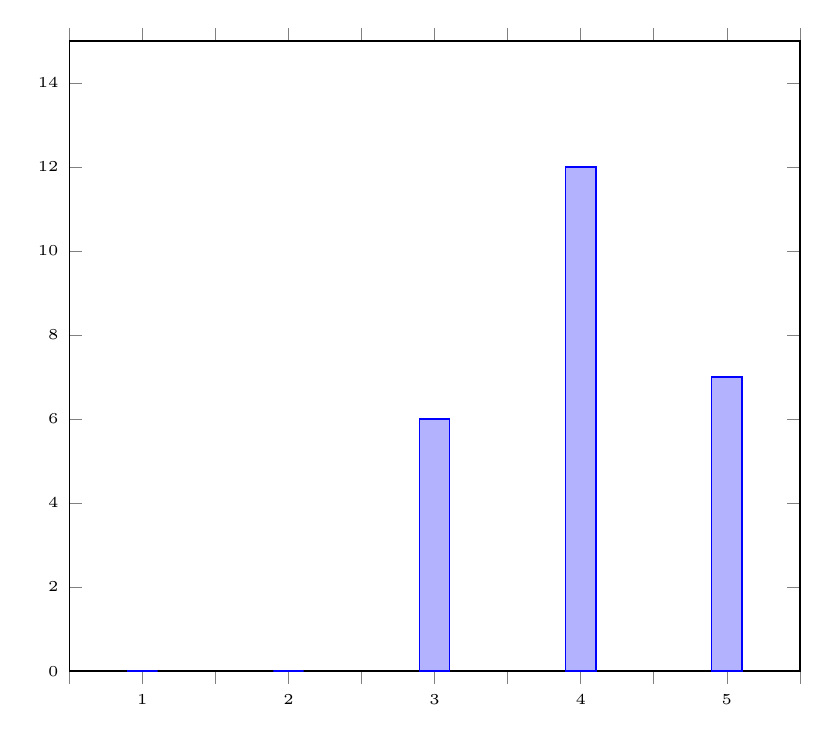
\begin{tikzpicture}[scale=1.1]

\begin{axis}[
style={font=\tiny},
ybar,
scale only axis,
xmin=0, xmax=20,
xticklabels={, ,$1$, ,$2$, ,$3$, ,$4$, ,$5$},
ymin=0, ymax=15,
]

\addplot coordinates{ (2,0) (6,0) (10,6) (14,12) (18,7)};

\end{axis}
\end{tikzpicture}
\caption{How likely participants would move an advertisement for later viewing}
\label{q6}
\end{center}
\end{figure}

\begin{figure}
\begin{center}
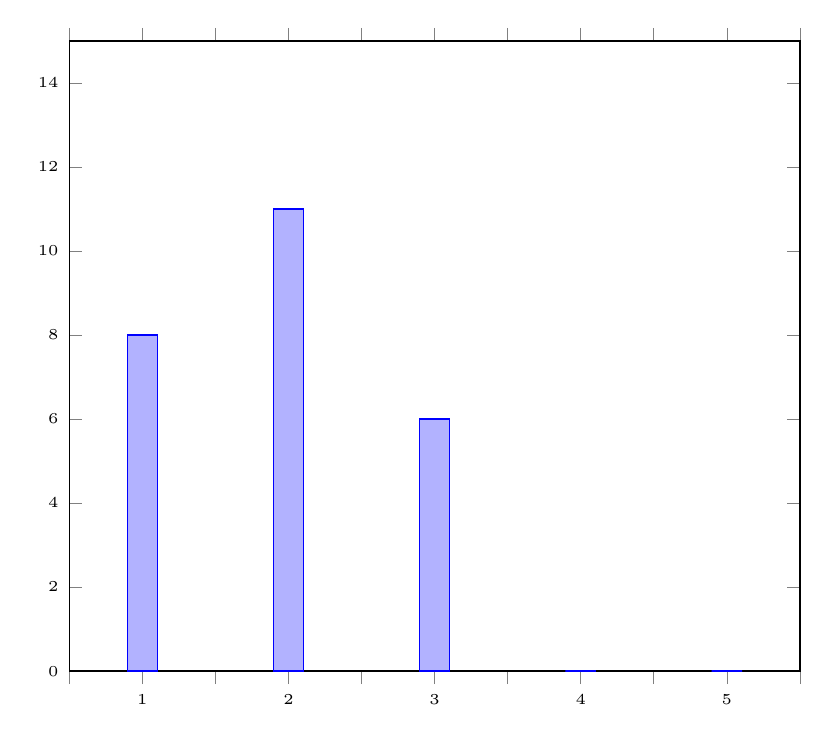
\begin{tikzpicture}[scale=1.1]

\begin{axis}[
style={font=\tiny},
ybar,
scale only axis,
xmin=0, xmax=20,
xticklabels={, ,$1$, ,$2$, ,$3$, ,$4$, ,$5$},
ymin=0, ymax=15,
]

\addplot coordinates{ (2,8) (6,11) (10,6) (14,0) (18,0)};

\end{axis}
\end{tikzpicture}
\caption{How likely participants would get rid of an advertisement as soon as it appeared}
\label{q7}
\end{center}
\end{figure}

When asked how they themselves think advertisements should be displayed in applications to make them less disruptive, the most common answers were that the advertisements should be smaller, blend in with the surroundings more and not be on top of content.

As seen from this feedback, the users would, at least some of the time, be willing to use the functionality this library provides for advertisements. Also, it has many of the features the users themselves proposed for making adverts more user friendly, like being smaller and not being on top of content the users wishes to interact with.

\section{Participants' Opinion of Dynamic Advertisements}

In terms of intrusiveness, all participants thought that the proposed method is less or just as intrusive as the classical method of advertisement delivery. 24\% thought that it is considerably less intrusive and 36\% that is just as intrusive as seen on Figure \ref{q8}.

\begin{figure}
\begin{center}
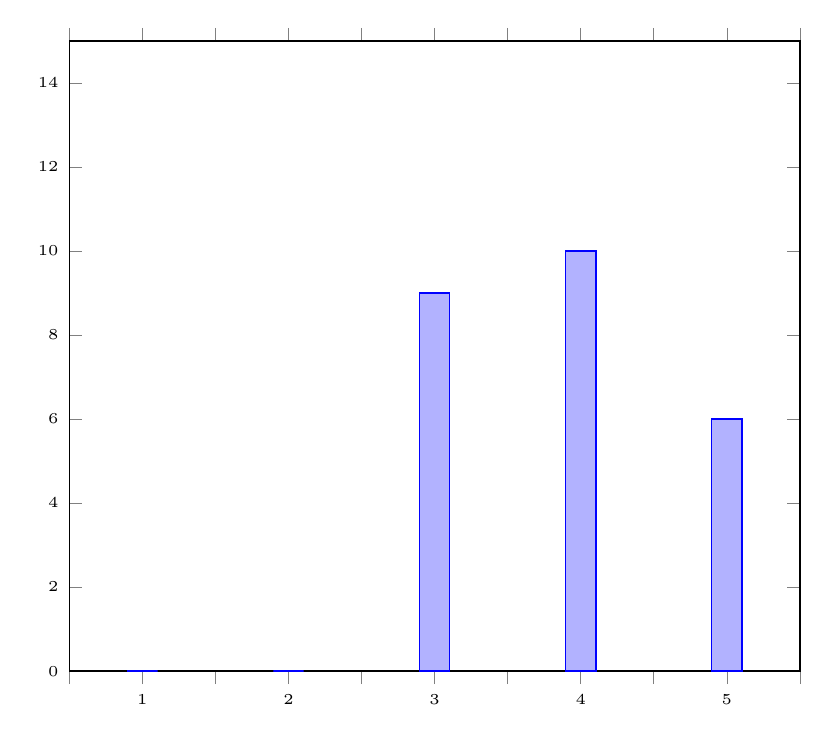
\begin{tikzpicture}[scale=1.1]

\begin{axis}[
style={font=\tiny},
ybar,
scale only axis,
xmin=0, xmax=20,
xticklabels={, ,$1$, ,$2$, ,$3$, ,$4$, ,$5$},
ymin=0, ymax=15,
]

\addplot coordinates{ (2,0) (6,0) (10,9) (14,10) (18,6)};

\end{axis}
\end{tikzpicture}
\caption{Intrusiveness comparison}
\label{q8}
\end{center}
\end{figure}

48\% of participants were just as interested in the advertised product as they would have been with the classical advertising method. 40\% were a little bit more interested and the product. 12\% were considerably more interested as seen on Figure \ref{q9}.

\begin{figure}
\begin{center}
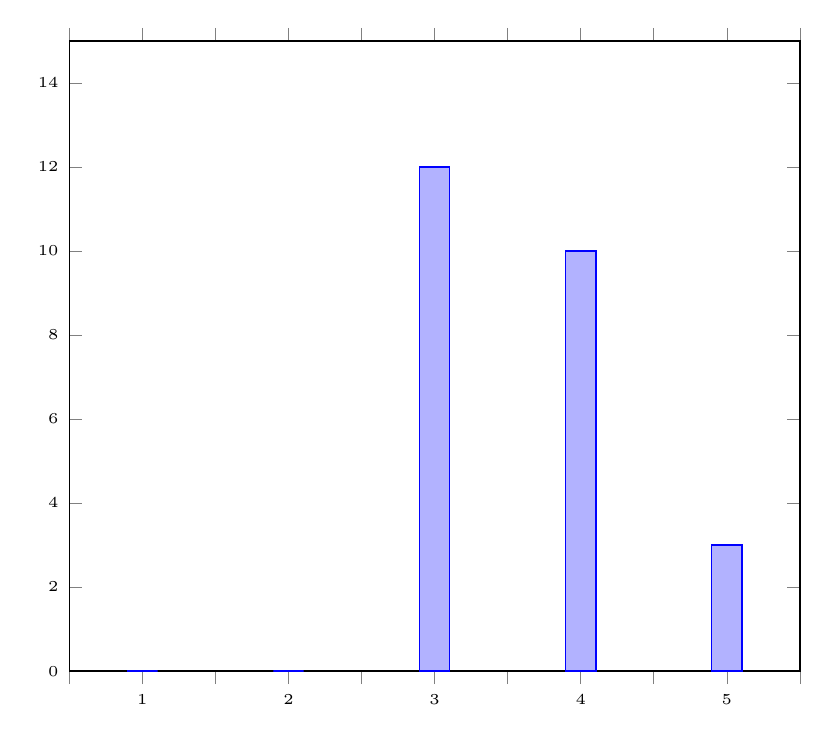
\begin{tikzpicture}[scale=1.1]

\begin{axis}[
style={font=\tiny},
ybar,
scale only axis,
xmin=0, xmax=20,
xticklabels={, ,$1$, ,$2$, ,$3$, ,$4$, ,$5$},
ymin=0, ymax=15,
]

\addplot coordinates{ (2,0) (6,0) (10,12) (14,10) (18,3)};

\end{axis}
\end{tikzpicture}
\caption{Interest comparison}
\label{q9}
\end{center}
\end{figure}

The general rating participants gave to the method of advertisement delivery is 3.96 on a scale from 1 to 5 as seen on Figure \ref{q10}.

\begin{figure}
\begin{center}
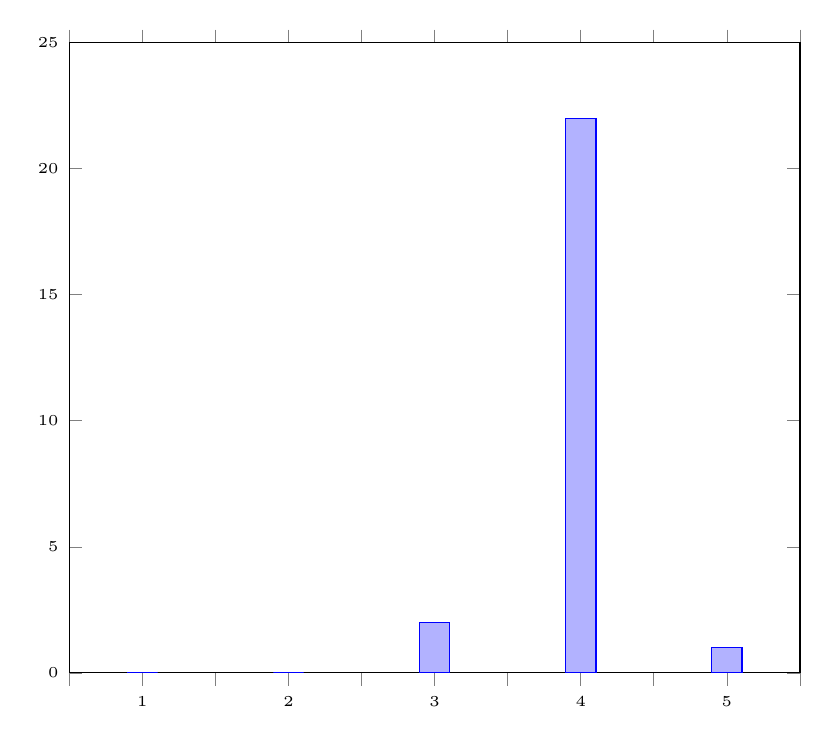
\begin{tikzpicture}[scale=1.1]

\begin{axis}[
style={font=\tiny},
ybar,
scale only axis,
xmin=0, xmax=20,
xticklabels={, ,$1$, ,$2$, ,$3$, ,$4$, ,$5$},
ymin=0, ymax=25,
]

\addplot coordinates{ (2,0) (6,0) (10,2) (14,22) (18,1)};

\end{axis}
\end{tikzpicture}
\caption{Rating}
\label{q10}
\end{center}
\end{figure}

\section{Summary}

In this chapter the usage of the proposed mechanism is validated. Based on the results, 64\% of the participants found the mechanism to be less intrusive than classical advertising. 52\% of the participants reported being more interested in the advertised product.

Almost all users found that being able to move an advertisement around on the screen is something that they would like to do in mobile applications. Some found that, being used to classical advertisements, the fact that the advertisement can be interacted with is not very intuitive and needs instructions on first application launch.

Some of the participants are application developers and were more than happy to start using this method for application monetization if it ever became a feasible option.